%% -*- mode: poly-noweb+R; ess-indent-level: 2; -*-

\chapter{Türelmetleneknek}

\section{Installálás}
\label{sec:1.1}


A mellékelt fileok között megtalálhatóak a \code{comproxy}, \code{com}
ill. \code{Rxls} csomagok win-binary formátumban. A telepítést ebben a
sorrendben kell elvégezni, pl. a menü használatával.   
A \code{comproxy} és \code{com} csomagok telepítését rendszegazdaként célszerű
elvégezni, és rögtön a telepítés után érdemes regisztrálni az \code{R}
\code{com} szerverét. 

A regisztráció csak akkor sikerül, ha rendszergazda jogosultsággal
hajtjuk végre. Pontosabban a \code{com} csomag regisztrációjának
elvégzéséhez, az \code{R} programot az ikon felett a jobb 
egérgombra klikkelve, a \code{Futtatás rendszergazdaként} lehetőséget
kiválasztva kell elindítani, lásd \aref{fig:1.1} ábrán.
\begin{figure}[h]
  \centering
  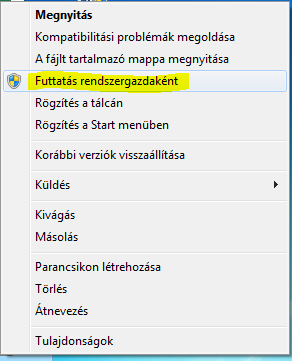
\includegraphics[width=16em]{images/start-as-root}
  \caption{R indítása rendszergazdaként.}
  \label{fig:1.1}
\end{figure}

A \code{comCheckRegistry} függvény ellenőrzi a registry bejegyzést,
lásd a \ref{sec:10.1} szakaszt.
\begin{Rnw}
<<echo=FALSE,results="hide">>=
suppressPackageStartupMessages(require(Rxls))
@ 
<<>>=
comRegisterRegistry()
comCheckRegistry()
@ 
\end{Rnw}
Az \code{Rxls} csomag telepítéséhez nem szükséges rendszergazdai
jogosultság.
Miután ennek telepítése is megtörtént, be kell tölteni az \code{Rxls}
csomagot
\begin{Rnw}
<<echo=FALSE,results="hide">>=
suppressWarnings(closeAllExcel())
unloadNamespace("Rxls")
unloadNamespace("com")
unloadNamespace("comproxy")
unlink(file.path(Sys.getenv("appdata"),"Rxls"),recursive=T)
##rm(list=ls(all=T))
@ 
<<>>=
require(Rxls)
installRxls()
@   
\end{Rnw}
A betöltés során valószínűleg kapunk egy figyelmeztetést, hogy az
\code{installRxls()} parancsot érdemes lefuttatni. Ez egyrészt létrehozza
az \code{\{APPDATA\}/Rxls} könyvtárat és ide másolja
a \code{R.xls}, \code{Rdev.xlam} és \code{Calc.xlt} munkafüzeteket
valamint létrehozza a verzió információt tartalmazó \code{versions} nevű file-t.
Alternatív lehetőség a mellékelt \code{R-COM\_setup\_x.x-x.exe}
legfrisseb változatának használata.

\section{\code{EXCEL} használata \code{R}-ből és fordítva}
\label{sec:1.2}

Tegyük fel, hogy az \code{Rxls} csomag telepítése sikeresen
megtörtént, az \code{installRxls} hiba nélkül 
lefutott. Elsőként az \code{Rdev.xlam} munkafüzetet érdemes
megnyitni. Ha rendszeresen használjuk bővítményként is telepíthetjük,
ekkor nem kell mindig megkeresni és betölteni. 

Az \code{Rdev.xlam} munkafüzet az alábbi címen lálható
\begin{verbatim}
<USER>/<APPDATA>/Rxls/Rdev.xlam
\end{verbatim}
Alapértelmezésben az \code{\{APPDATA\}} könyvtár rejtett. Ezt a vezérlő
pult használatával felfedhetjük (rejtett mappák megjelenítése). Másik
lehetőség, hogy a windows intéző címsorába 
beírjuk az elérési utat. \code{R}-ből a pontos elérési utat az appdata
környezeti változóból is kiolvashatjuk: 
\begin{Rnw}
<<>>=
Sys.getenv("appdata")
@  
\end{Rnw}
Ez egyben az első tesztje annak, hogy az elképzelt mechanizmus
működik-e más gépeken is. Az \code{Rdev.xlam} megnyitásakor az
\code{EXCEL} megpróbálja megnyitni a hivatkozott \code{R.xls} 
munkafüzetet is. Egyáltalán nem nyivánvaló, hogy ez sikerül is,
ugyanis az \code{EXCEL} a teljes elérési utat megjegyzi, ami nyilván
nem létezik, ha a munkafüzetet egy másik gépre visszük 
át. Ezért a \code{Workbook\_open} rutin ellenőrzi, hogy létezik-e
megnyitott \code{R.xls} munkafüzet. Ha 
nincs ilyen nevű munkafüzet megnyitva, akkor megpróbálja megnyitni az
\code{\{appdata\}/Rxls} könyvtárból. Ha telepítés rendben megtörtént,
akkor ez sikerül is. 
Ha minden rendben ment, akkor az újabb, ribbon-t használó \code{EXCEL}
változatok esetén a Bővítmények fül alatt, régebbi \code{EXCEL}
változatok esetében pedig a menüsorban megjelenik két 
almenü, az egyik felirata \code{R}, a másiké \code{Rxls development}.
A telepítés legegyszerűbb tesztelése, ha ráklikellünk az
\begin{verbatim}
R->R ablak megjelenítés
\end{verbatim}
menüpontra. Hatására az \code{EXCEL} megnézi, hogy van-e futó \code{R}
alkalmazás, ha van akkor az 
láthatóvá válik, ha nincs akkor elindít egy új \code{R} példányt. A
következő lépés az \code{R} és \code{EXCEL} 
összekötése az
\begin{verbatim}
R -> R<->EXCEL összekötés
\end{verbatim}
menüponttal. Ez az \code{EXCEL} új Ribbon kezelő felületén a
\code{Bövítmények} fül alatt van, de elérhető az \code{Rxls
  development} fülön is. Ennek hatására az \code{R} oldalon létrejön
egy változó \code{THISXL} névvel. Ez reprezentálja az \code{EXCEL}
alkalmazást.  Pontosabban ez a változó a \code{.XL<azonosító>} nevű
környezeten belül jelenik meg. Ahhoz, hogy az \code{Rxls} csomag
rutinjai is ``lássák'' a keresési útvonalhoz is csatoljuk. Ennek a
megoldásnak az az előnye, hogy a kapcsolat bontásakor (azaz az EXCEL
bezárásakor egyszerűbben lehet az adott EXCEL példányra történő
hivatkozásokat törölni). 

% Ezt láthatóvá kell tenni az \code{Rxls}
%csomag rutinjai számára. Vagy a globális környezetbe kell másolni, vagy
%csatolni kell a keresés útvonalhoz. 
\begin{Rnw}
<<echo=FALSE,results="hide">>=
suppressPackageStartupMessages({require(com);require(Rxls)})
getExcelWithRdev(NULL)
cmd<-withObj(THISXL,{
                 ##if(.$workbooks()$count()==0)
                 ## .$workbooks()$add()
                 ##.$run("R.RIC.connect",TRUE) 
                 ## Sys.sleep(.1)
                 cmd<-.$run("R.RIC.defaultcmd")
                 cmd2<-change.cmd(cmd,fun="ls.str",
                                  keep=c("envir"="env"),all.names=TRUE)
                 cmd1<-sub("[$]wb_[^,]*," , "," , cmd2)
                 cmd3<-"ls.str(2,all=TRUE)"
                 cmd4<-"search()[1:5]"
                 ##cmd5<-"THISXL"
                 paste(cmd1,cmd2,cmd3,cmd4,##cmd5,
                       sep="\n")
             })

## acmd<-change.cmd(cmd,
##            fun="with",
##            keep=c(env="envir"),
##            expr=substitute(attach(list(THISXL=THISXL,
##            .wbname=.wbname,.wsname=.wsname),
##            name="XL")))

#xlins<-ls(all=T,pattern="^.XL",envir=.GlobalEnv)
#assign(xlins,get(xlins,.GlobalEnv))
#rm(xlins)
@ 
<<code=cmd>>=
@ 

<<echo=FALSE,results="hide",eval=FALSE>>=
safe.detach("XL")
local({
    cmd<-change.cmd(cmd,fun="eval",
                    keep=c(expr="envir"),
                    env=substitute(.GlobalEnv))
    xlenv<-eval(parse(text=cmd))
    attach(with(xlenv,list(THISXL=THISXL)),name="XL")
})
##rm(list=ls(all=TRUE))
@ 
\end{Rnw}
Ennek segítségével ugyanúgy használhatjuk a hivatkozott \code{EXCEL} példányt \code{R}-ből, mint
Visual Basic-ből. Például, létrehozhatunk egy új munkafüzetet és abban
az \code{\$A\$1} cellát kitölthetjük értékkel, vagy formulával. A
formátum első ránézésre talán szokatlan. Ahol a 
Visual Basic kódban pont van, ott vagy egy tulajdonságot kérdezünk le,
vagy egy metódust alkalmazunk. A \code{com} csomag korábbi változataiban a
két esetnek eltérő a szintakszisa: 
tulajdonságot
$$
\code{obj[[<tulajdonságnév>, <argumentumok>]]},
$$
míg metódust
$$
\code{obj\$<metódusnév>(<argumentumok>)}
$$
alakban lehet elérni. Az új változatban, \code{1.0-52}-től felfelé,
lehetőség van a \code{<obj>\$<név>()} 
szintakszis használatára tulajdonság lekérdezés esetén is, lásd a
\ref{sec:10.1} szakaszt. 
\begin{Rnw}
<<hibas>>=
wb<-THISXL[["workbooks"]]$add()
cell<-wb[["sheets",1]][["range","$A$1"]]
cell[["value"]]
cell[["value"]]<-1
cell[["value"]]
cell<-cell$offset(1,0)
cell[["formula"]]<-"=$A$1+2"
cell[["formula"]]
cell[["value"]]
cell<-NULL
@
\end{Rnw}
Az \code{Rxls} csomag célja, hogy a gyakran elő forduló adatmozgatásokat
egyszerűen  lehessen végrehajtani. Pl. adott \code{EXCEL} tartomány értékét az
\code{XLget} függvénnyel is elérhetjük. Az 
\code{XLreaddf} és \code{XLwritedf} függvények \code{data.frame}-t
olvasnak be ill. írnak \code{EXCEL} tartományból, 
ill. tartományba. 
\begin{Rnw}
<<>>=
df <- data.frame(Dátum = seq.Date(as.Date("2012-01-01"),
by = "1 month", length = 5))
df$díj <- rnorm(nrow(df), 100)
df$kárkifizetés <- rnorm(nrow(df), 70)
df
XLwritedf(XLrange = THISXL[["range", "$C$1"]], df = df,
with.names = TRUE, autoFit = TRUE, setname = "havi_bontás")
@  
\end{Rnw}
Az utolsó sor hatására az \code{EXCEL} aktív munkalapjára másolódik a \code{df}
\code{data.frame} a változónevekkel együtt (ez a táblázat felső sora lesz),
az oszlop szélességeket az éppen másolt 
táblázathoz illesztjük, végül létrehozunk egy nevet az aktív
\code{EXCEL} munkafüzetben, ami arra a tartományra hivatkozik, ahová
az adatokat másoltuk. 
\begin{Rnw}
<<>>=
## wb a korábban létrehozott új munkafüzet
address<-wb[["names"]]$item("havi_bontás")[["refersto"]] #$
address
df1<-XLreaddf.cols(address)
df1
## vagy
range<-wb[["names"]]$item("havi_bontás")[["referstorange"]] 
range$address(external=TRUE) 
df2<-XLreaddf.cols(XLrange=range)
identical(df1,df2)
@ %$
<<echo=FALSE,results="hide">>=
range<-NULL
wb$close(FALSE) 
wb<-NULL
rm(range,wb,address,cell)
gc()
@ %$
\end{Rnw}
Látható, hogy a dátum adatok részben elvesztek. Ennek az az oka, hogy
az \code{XLreaddf.cols} 
ill. \code{XLreaddf.rows} függvények a tartomány \code{value2}
tulajdonságát használják. Amikor ezek 
a rutinok születtek a \code{com} (lánykori nevén \code{rcom}) nem
tudta kezelni a dátum típusú adatokat. 
Kerülő megoldásként született az \code{XLDate} függvény, ami a
numerikus adatot visszaalakítja \code{Date} típusúvá.
\begin{Rnw}
<<>>=
XLDate(df1$Dátum) 
@  %$
<<echo=FALSE,results="hide">>=
rm(df,df1,df2)
@
\end{Rnw}

\section{Egyszerű minta projekt}
\label{sec:1.3}


\begin{Rnw}
<<echo=FALSE,results="hide">>=
msg<-function(...) {
  cat("\n",sprintf(...),"\n",sep="");
  flush.console()
}

getExcelWithRdev(NULL,new=TRUE)

msg("XL ribbon visible")
withObj(THISXL,{
  Sys.sleep(2)
  .[["visible"]]<-TRUE;
  .[["top"]]<-0;
  .[["left"]]<-0
  .[["height"]]<-190
  .$range("$A$1")$select()
})
setRibbon(THISXL,hide=TRUE)
setRibbon(THISXL,hide=FALSE,extraKeys="%y{ESCAPE}{ESCAPE}")
##{ESCAPE}{ESCAPE}")
capturewnd("Rxls_development_menu.bmp")
setRibbon(THISXL,hide=TRUE)

msg("XL 'newskeleton'")
THISXL$run("Rdev.xlam!newskeleton") #,fp("Calc1"))
Sys.sleep(2)
wb<-THISXL$activeworkbook();

withObj(wb$activesheet(),{
  msg("XL 'Adatok' worksheet")
  withObj(.$range("B5:B7"),{
    .$select()
    THISXL$run ("Rdev.xlam!insertDataLine");
    Sys.sleep(.5)

    .[["value"]]<-as.XLdata(list("Technikai kamat","Nem","Eredmény helye"))
  })
  withObj(.$range ("A5:A7"),
  .[["value"]]<-as.XLdata(list ("i","nem","wsname"))
  )

  withObj(.$range ("C6"),{
    .[["value"]]<-"férfi;női"
    .$select ()
  })
  THISXL$run ("Rdev.xlam!insertDropDown");
  Sys.sleep(.5)

  withObj(.$range("E5:E6"),
  .[["value"]]<-as.XLdata(list(0.05,"férfi")))

  withObj(.$range("E7"),
  .[["formula"]]<-'="Komm. számok ("&D6&",i="&D5&")"')

  .$range ("C6")$select ()
})

msg("XL 'adatok.bmp'")
withObj(THISXL,{
  .[["height"]]<-245
  .[["width"]]<-680
})
capturewnd("adatok.bmp")

local({
  cmd<-THISXL$activesheet()$shapes(1)$onaction()
  Sys.sleep(.1)
  suppressMessages(THISXL$run(cmd,TRUE))
  Sys.sleep(.1)
})

msg("XL inserting lx")
lx2003<-read.csv("lx2003.txt",sep=";")

withObj(wb$worksheets()$add(),{
  .[["name"]]<-"lx"
  XLwritedf(XLrange=.$range("A1"),df=lx2003)
  wb$names()$add(name="lxdata",refersto=.$usedrange())
})

withObj(wb$worksheets("R kód"),{
  .$activate()
  .$names("R_data")$referstorange ()$select()
})

withObj(THISXL,{
  .[["height"]]<-170
  r<-.$selection()
  withObj(.$activewindow(),{
    .[["scrollcolumn"]]<-r$columns(1)$column()
    .[["scrollrow"]]<-r$rows(1)$row()
  })
})
capturewnd("R-kod.bmp")
@
\end{Rnw}

%%% Local Variables: 
%%% mode: latex
%%% TeX-master: "Rxls"
%%% End: 


Tegyük fel, hogy van egy \code{R} scriptünk \code{calc.R} névvel.
\begin{Rnw}
<<>>=
cat(readLines("calc.R"), sep = "\n")
@  
\end{Rnw}
Ez a script kommutációs számokat számol módosított halandósági
táblából, a halálozási 
rátát módosítjuk az eredeti 95~\%-ára. A \code{calc.cn} függvénynek
három argumentuma van, 
ebből legalább kettőt kell megadni, az \code{lx} halandósági függvényt és a \code{nu} diszkont ráta ill.
\code{i} technikai kamat közül az egyiket, vagy mindkettőt. Ez a
számolás csak a diszkont rátát 
használja, de az ereményben megjegyezzük a technikai kamatot, azaz
\code{i}-t is.
\begin{Rnw}
<<>>=
source("calc.R", local = TRUE)
str(cn)
@
\end{Rnw}
Tegyük fel, hogy a bemenő adatokat \code{lx}, \code{nu} és \code{i}-t
szeretnénk \code{EXCEL}-ben beállítani és az 
eredményül kapott táblázatot a számoló munkafüzet új lapjára
szeretnénk írni. A \code{lx} halandósági függvény az \code{EXCEL} három oszlopos
táblázata, kor, férfi és női oszlopokkal. Azt 
szeretnénk, hogy a számoló munkafüzetben be lehessen állítani, a
technikai kamat értékét, 
azt, hogy férfi, vagy női haladósággal akarunk számolni, valamint azt
is, hogy mi legyen az 
új munkalap neve.

A megvalósításhoz nyissuk meg az \code{Rdev.xlam} munkafüzetet. Ha
nincs beállítva, akkor engedélyezzük a \code{Visual Basic}
projektekhez való hozzáférést. Hozzunk létre egy új számoló 
munkafüzetet az \code{Rxls development} menü \code{Új számoló munkafüzet}
parancsával. A felugró 
mentés ablakban adjuk meg az új munkafüzet nevét, alapértelmezésben
\code{Calc1.xls}. A fileformátum lehet \code{xlsm} is. Az új
munkafüzetben két lap van \code{Adatok} ill. \code{R kód} névvel. 
Első lépésben az \code{Adatok} munkalapot töltsük fel. A jobb egérgomb
alatti menüben az 
\code{Insert Form} pont alatt található néhány gyakrabban előforduló elem.

Jelöljük ki a \code{\$B\$5:\$B\$7} tartományt és a jobb egérgomb alatt
felnyíló menüt használva 
illesszünk be egy \code{Data Line}-t. A \code{\$B} oszlopban cseréljük
le az \code{Adat} neveket a következőkkel: \code{Technikai kamat},
\code{Nem} és \code{Eredmény helye}. Töltsük ki az \code{\# R nevek
  \#} oszlopot \code{i}, \code{nem}, \code{wsname}-mel. Ezek lesznek a
változó nevek az \code{R} oldalon. 
Ezután adjuk meg az alapértelmezett értékeket: a technikai kamat
esetén ez lehet pl. 0.02 a nem esetén férfi, míg az Eremény helye mező
esetén lehet egy képlet, ami a technikai 
kamat és a nem értékéből kiszámolja az új munkalap nevét, pl.
\begin{VBAframe}
="Komm. számok("\&\$D\$6\&",i="\&\$D\$5\&")"
\end{VBAframe}
Végül mivel a \code{Nem} mező esetén csak két lehetséges értékből
lehet választani, töltsük ki a \code{\$C\$6} mezőt \code{férfi;női} értékkel. Ez a választható értékek felsorolása pontosvesszővel elválasztva. Ha most kijelöljük a \code{\$C\$6} mezőt és a jobb egérgomb alatt felnyíló menü segítségével 
beszúrunk egy \code{Drop Down Data}-t, akkor az \code{R} kód
munkalap \code{\$A} oszlopának aljára másolódik a lehetséges értékek
listája, és a \code{\$C\$6} cellában megjelenik egy lenyíló vezérlő
elem. A vezérlő elem alatt a \code{\$C\$6} cella zárolt lesz, és a
képletezés hatására mindig a választott értéket 
tartalmazza.

Az így kialakított munkalap képe \aref{fig:1.2} ábrán látható. 
%1.2. ábra. Adatok munkalap
\begin{figure}[h]
  \centering
  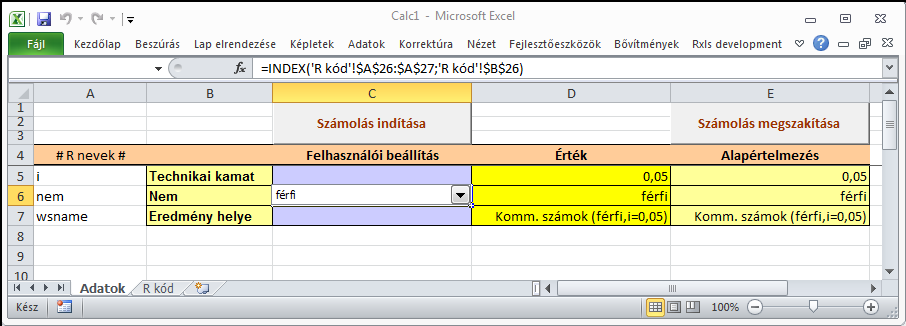
\includegraphics{images/adatok}
  \caption{\code{Adatok} munkalap}
  \label{fig:1.2}
\end{figure}

Ha ezen a ponton a \code{Számolás indítása} gombra klikkelünk, akkor
az \code{Adatok} munkalapon definiált változók megjelennek az \code{R}
oldalon is. Ezt ellenőrizhetjük az \code{ls.str()} parancs 
beírásával az \code{R} konzolba. A \code{R} ablakot az \code{EXCEL}
\begin{verbatim}
Bővítmények -> R -> R ablak megjelenítése
\end{verbatim}
menüponttal jeleníthetjük meg, ha az háttérben van.
\begin{Rnw}
<<echo=FALSE,results="hide">>=
cmd<-local({
  cmd<-THISXL$run("R.RIC.defaultcmd")
  Sys.sleep(.1)
  change.cmd(cmd,fun="ls.str",keep="env",all.names=TRUE)
})
@
<<code=cmd>>=
@
% XLid<-ls(pos=1,pattern="\\.XL[0-9]+",all=T)
% XLid
% ls.str(XLenv<-get (XLid,pos=1))
% wbid<-ls(envir=XLenv,pattern="wb_Calc")
% ls.str(get(wbid,envir=XLenv))
\end{Rnw}
A \code{Számolás indítása} gomb megnyomásakor annyi történt, hogy az
\code{EXCEL} az \code{R} oldalon létrehozott egy környezetet, ami az
adott \code{EXCEL} példány és aktív munkafüzet adatait tartalmazza:
hivatkozás az \code{EXCEL.Application}-ra és a munkafüzet neve, és
ebben a környezetben végrehajtotta a \code{R kód} munkalapon
összerakott kódot. Ez ezen a ponton egyetlen utasítást tartalmaz, ami
a \code{\_Rdata} tartomány (ez az \code{Adatok} munkalap első négy
oszlopa) első oszlopából a változó neveket, a 4. oszlopából az
értékeket veszi.  
\begin{figure}[h]
  \centering
  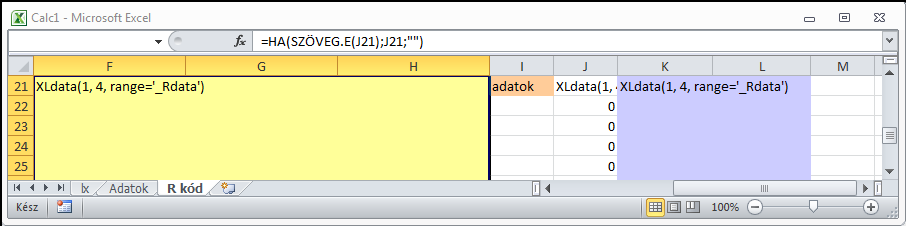
\includegraphics{images/R-kod}
  \caption{Az \code{'R kód'} munkalap részlete}
  \label{fig:1.3}
\end{figure}


Ezzel persze még a számolást nem tudjuk elvégezni, mert nem adtuk át a
halandósági függvényt \code{lx}-et, amire szintén szükség van a
számoláshoz. Ha ezt is az \code{EXCEL} munkafüzetben 
szeretnénk tárolni, akkor illesszük be egy új munkalapra. Az \code{R}
kódot úgy fogjuk módosítani, hogy a halandósági táblát a munkafüzet
\code{lxdata} nevű tartományából vegye. Ezért a halandósági táblát
tartalmazó tartománynak adjuk meg ezt a nevet az \code{EXCEL}
névkezelőjében.

%  és lépjünk át
% az \code{R kód} munkaplapra. Keressük meg az adatok megadására szolgáló
% részt, lásd az \ref{fig:1.3} ábrán. 
% %1.3. ábra. R kód munkalap

% A változtatásokat 
% ezen a munkalapon a kékes színű mezőkbe érdemes írni, a munkalap többi
% része úgy van 
% képletezve, hogy az itt megadott adatokból összerakja a végrehajtandó \code{R} kódot. Az első sor
% ki van töltve ez mondja meg az \code{R}-nek, hogy olvassa be az adatok
% munkalapon megadott adatokat. A második sor fogja megmondani az
% \code{lx} tartomány nevét. Mivel \code{EXCEL} tartományok 
% teljes címére gyakran van szükség az \code{R.xls} munkafüzetben
% definiálva van az \code{extAddress} 
% munkalapfüggvény, ami az első argumentumának címét adja vissza
% szöveges formátumban, 
% ha a második argumentum \code{IGAZ}, akkor a aposztrófok
% között. Emellett szükség van annak 
% a munkafüzetnek a nevére is, amibe az eredményt be akarjuk
% illeszteni. Ez a mi esetünkben a \code{Calc1.xls} munkafüzet, ezért a
% harmadik sorban \code{wbname<-"Calc1.xls"} kerül. Ez is 
% képletezve van, így a munkafüzetet akár más néven is elmenthetjük.

Utolsó lépésként meg kell adnunk a \code{Calc1.xls} munkafüzetben azt
is, hogy az \code{R}-nek átadott adatokkal milyen számolást is végezzen. Ha
hordozhatóvá akarjuk tenni a munkafüzetet, akkor erre a legegyszerűbb
megoldás, ha a számolást végző \code{R} kódot is a munkafüzetben 
tároljuk. Ezt \code{R kódlap} beszúrásával tehetjük meg.
A \code{calc.R} közvetlenül nem alkalmas a céljainkra, a szkript végét
módosítani kell, hogy a számolást 
az \code{EXCEL}-ből kapott adatok alapján végezze. A módosított és az
eredeti  \code{R} szkript is megtalálható a 
mellékelt file-ok között.
\begin{Rnw}
<<echo=FALSE,results="hide">>=
writeLines(readLines("../aux/calc1.R",encoding="UTF-8"),sep="\n",con="calc1.R")
@
<<>>=
calc.R <- readLines("calc.R")
calc1.R <- readLines("calc1.R")
cat("új sorok:", setdiff(calc1.R, calc.R), "\ra régi helyett:",
                 setdiff(calc.R, calc1.R), sep = "\n")
@
\end{Rnw}
Az így módosított kódot szúrjuk be \code{R kódlap}-ként a
munkafüzetbe. Az \code{R kódlap beszúrás} funkciót két helyen is
megtalálhatjuk, egyrészt az \code{Rxls development} menüpont alatt,
másrészt a munkalap fülekről felnyíló menüben is. A művelet
eredményeként egy új munkalap jön létre \code{R kód(calc1.R)} névvel,
lásd az \ref{fig:1.4} ábrát.
\begin{figure}[h]
  \centering
  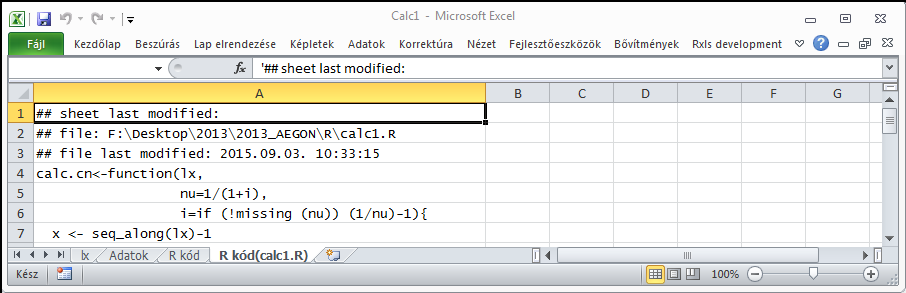
\includegraphics{images/R-kod_calc1R}
  \caption{Az \code{'R kód(calc1.R)'} kódlap}
  \label{fig:1.4}
\end{figure}

Ezután be kell jegyezni az \code{R kód} munkalapon, hogy a
\code{calc1.R} kódlapot az \code{R}-nek végre 
kell hajtania. Ehhez az \code{R kód} munkalapon töltsük ki a kódlapok
mező első sorát az \ref{fig:1.5} ábrán látható módon.
\begin{figure}[h]
  \centering
  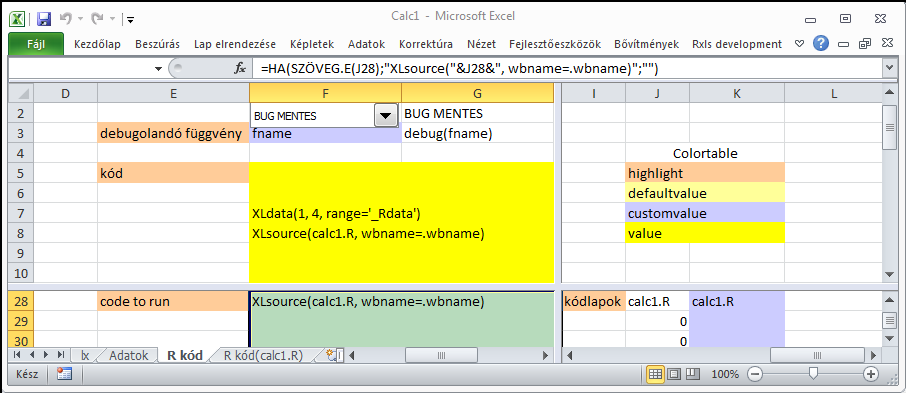
\includegraphics{images/R-kod-filled}
  \caption{Az \code{'R kód'} munkalap kitöltve}
  \label{fig:1.5}
\end{figure}

Ezzel a \code{Calc1.xls} munkafüzet elkészült. Utolsó lépésként kattintsunk a
\begin{verbatim}
Bővítmények -> Rxls development -> Véglegesítés
\end{verbatim}
gombra. Ekkor az \code{R kód} nevű munkalapok eltűnnek, az
\code{Adatok} munkalapon az első oszlop 
elrejtődik, és a látható munkalapok védetté válnak. Ezután csak a
kékes színű felhasználói 
adatok részére fenntartott mezőkbe lehet írni.


\begin{Rnw}
<<echo=FALSE,results="hide">>=
withObj(wb$worksheets("R kód")$names("R_calc")$referstorange ()$offset (0,3),
.[["value"]]<-"calc1.R")

THISXL$run("Rdev.xlam!insertRcode",fp("calc1.R"),wb)
Sys.sleep(.5)

withObj(THISXL,{
  .[["height"]]<-220
  capturewnd("R-kod_calc1R.bmp")

  .[["height"]]<-295
  withObj(wb$worksheets("R kód"),{
    .$activate()
    .$names("R_calc")$referstorange()$select()
  })
  withObj(.$activewindow(),{
    .[["scrollrow"]]<-2; 
    .[["scrollcolumn"]]<-4;
    .[["splitcolumn"]]<-4
    .[["splitrow"]]<-9
    withObj(.$panes(2), .[["scrollcolumn"]]<-9)
    withObj(.$panes(3),.[["scrollrow"]]<-28)
    capturewnd("R-kod-filled.bmp")
    .[["split"]]<-FALSE
  })
})

rm(list=ls(all=T))
gc()
@  

\end{Rnw}


%%% Local Variables: 
%%% mode: latex
%%% TeX-master: "Rxls"
%%% End: 

\endinput

\begin{Rnw}
<<>>=
ls(all=T)
ls(all=T,pos=1)
@
  
\end{Rnw}

%%% Local Variables: 
%%% mode: latex
%%% TeX-master: "Rxls"
%%% End: 
